\input{configuration}

\def\ojoin{\setbox0=\hbox{$\bowtie$}%
  \rule[-.02ex]{.25em}{.4pt}\llap{\rule[\ht0]{.25em}{.4pt}}}
\def\leftouterjoin{\mathbin{\ojoin\mkern-5.8mu\bowtie}}

\title{Tutorial 9 --- Isolation and Recovery }

\author{Richard Wong \\ \small \texttt{rk2wong@edu.uwaterloo.ca}}
\institute{Department of Electrical and Computer Engineering \\
  University of Waterloo}
\date{\today}


\begin{document}

\begin{frame}
  \titlepage

\end{frame}


\begin{frame}
\frametitle{Exercise 9-1}

For the following transaction schedule, fill in the RW-timestamps for data items $a$ and $b$, assuming we use the simple timestamp-ordering protocol.

How would the answer change if we used the Thomas Write Rule?

\begin{center}
\begin{tabular}{ | c c c || c c c c | }
  \hline
  $T_1$ & $T_2$ & $T_3$ & $TS_r(a)$ & $TS_w(a)$ & $TS_r(b)$ & $TS_w(b)$ \\
  \hline
  $r_a$ &       &       &           &           &           &           \\
        & $r_b$ &       &           &           &           &           \\
        &       & $r_a$ &           &           &           &           \\
  $w_a$ &       &       &           &           &           &           \\
        & $r_a$ &       &           &           &           &           \\
        &       & $w_b$ &           &           &           &           \\
  $r_b$ &       &       &           &           &           &           \\
        & $w_b$ &       &           &           &           &           \\
        &       & $w_a$ &           &           &           &           \\
  \hline
\end{tabular}
\end{center}

\end{frame}


\begin{frame}
\frametitle{Exercise 9-2}

Under what conditions does the phantom read phenomenon occur?

\end{frame}


\begin{frame}
\frametitle{Exercise 9-3}

Suppose we need to recover from a system failure, and have the transaction log below.

Assuming we use an immediate update protocol with checkpointing, what log entries does the recovery system need to add to restore the database to a consistent state?

\begin{center}
\begin{tabular}{ | l | c c c c | c | }
  \hline
  action & transaction & item & val & val' & flags \\
  \hline
  start & $T_1$ &   &   &   &           \\
  write & $T_1$ & a & 1 & 2 &           \\
  write & $T_1$ & a & 2 & 3 &           \\
  checkpoint & [$T_1$] &   &   &   &           \\
  want to abort & $T_1$ &   &   &   &           \\
  write & $T_1$ & a & 3 & 2 & redo-only \\
  start & $T_2$ &   &   &   &           \\
  write & $T_2$ & b & 5 & 6 &           \\
  write & $T_2$ & b & 6 & 7 &           \\
  (system failure) &       &   &   &   &           \\
  \hline
\end{tabular}
\end{center}

\end{frame}


\begin{frame}
\frametitle{Exercise 9-4}

Where do the following recovery protocols belong in the table below?

\begin{enumerate}
  \item deferred update
  \item immediate update (\textit{can} persist prior to commit)
  \item strict immediate update (persist changes immediately)
\end{enumerate}

\begin{center}
\begin{tabular}{ | l | c | c | }
  \hline
          & redo & no-redo \\
  \hline
  undo    &      &         \\
  \hline
  no-undo &      &         \\
  \hline
\end{tabular}
\end{center}

\end{frame}


\begin{frame}
\frametitle{Exercise 9-5}
  What data is logged in order for the ARIES protocol to restore from a checkpoint?
\end{frame}


\begin{frame}
\frametitle{Exercise 9-6}
  Suppose a checkpoint is made between LSN 7 and 8 in the following schedule.

  What data is stored in the transaction table and the dirty page table?

  Where should the REDO phase start scanning for operations?

  \begin{center}
  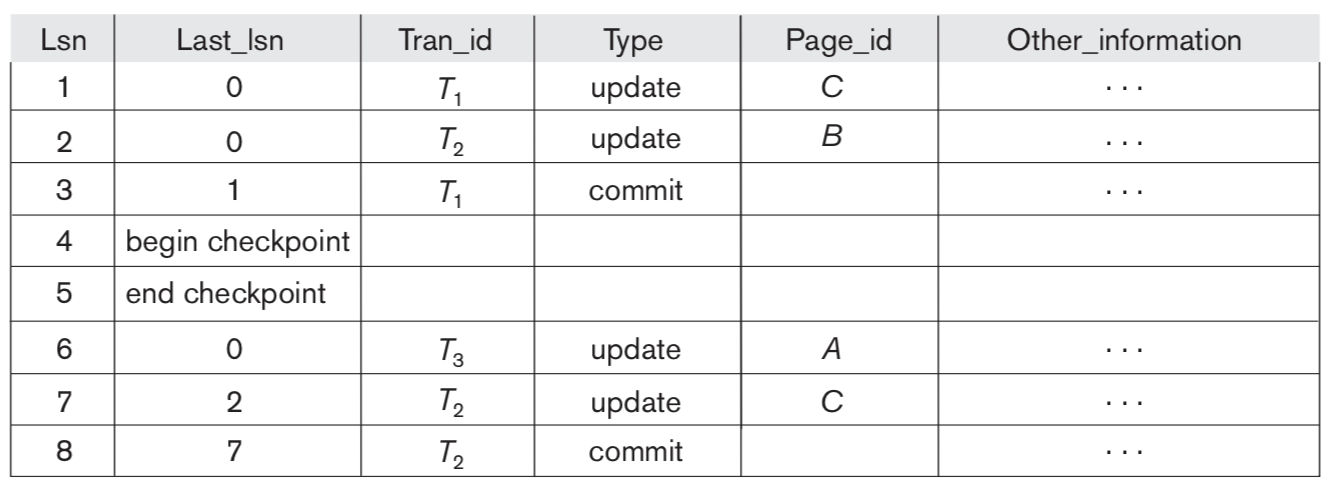
\includegraphics[width=0.85\textwidth]{images/aries-1}\\
  \end{center}
\end{frame}


\begin{frame}
\frametitle{Exercise 9-7}
  Why is it important for the ARIES protocol to look for the most recent \textit{end-checkpoint} log record as opposed to the most recent \textit{start-checkpoint} log record during its analysis phase (finding TT and DPT at last checkpoint)?
\end{frame}


\end{document}
